\chapter{Experimental Setup}
\label{chapt:experimental_setup}
In this Chapter, we outline the experimental setup used in this research to ensure transparency and reproducibility of the results. We begin with an overview of the hardware configuration in Section \ref{sec:hardware}, detailing the computational resources utilized, including CPUs, GPUs, and storage systems. Following this, Section \ref{sec:software} describes the software environment, highlighting the programming languages, libraries, and tools employed throughout the experiments. Next, Section \ref{sec:data} introduces the datasets used, specifically focusing on the basketball and soccer datasets. This Section details the data preprocessing steps necessary to convert them into a unified data structure, ensuring consistency in analysis. Subsequently, Section \ref{sec:experiments} presents an overview of the experiments conducted to evaluate the performance of various predictive models, discussing factors such as input data types, historical context, and forecast horizons. Finally, Sections \ref{sec:model_configurations} and \ref{sec:training_details} provide insights into the specific model configurations and training details respectively, which will guide the comprehensive evaluation of the models' capabilities across different~conditions.


\section{Hardware Configuration}
\label{sec:hardware}
The computational experiments were conducted on a high-performance cluster running CentOS Linux 7.9.2009 with kernel version 3.10.0-1160.71.1. The cluster consists of 8 \gls{gpu} nodes and 4 \gls{cpu} nodes. Each \gls{cpu} node is equipped with two Intel Xeon Gold 5120 processors, each featuring 28 cores and 2 threads per core, operating at a base frequency of 2.20 GHz. Each \gls{gpu} node contains two Intel Xeon Gold 5120 processors and four Tesla V100-SXM2 \glspl{gpu}, each with 32,768 MiB of dedicated memory.

\section{Software Configuration}
\label{sec:software}

This research employs Conda (version 23.10.0) as a crucial tool for managing software environments and dependencies. Conda simplifies the installation of required libraries, ensuring compatibility across a variety of computational tasks. The programming language Python (version 3.11.0) serves as the foundation for developing, testing, and benchmarking the machine learning models used in this study.

\parbox{\linewidth}{
        The \texttt{pyproject.toml} file for Gosalci's project \cite{Gosalci_master_den_2024} defines the essential Python packages needed for the project. These include \texttt{torch==2.4.1+cu118} for deep learning applications with CUDA support (version 11.8), \texttt{numpy==2.0.1} for efficient numerical operations, \texttt{pandas==2.2.2} for data processing and manipulation, \texttt{matplotlib==3.9.1.post1} for data visualization, \texttt{scipy==1.14.0} for scientific computing tasks, \texttt{Pillow==10.4.0} for image processing, \texttt{py7zr==0.21.1} for handling 7z archives, \texttt{codecarbon==2.5.1} for tracking carbon emissions from computations, \texttt{lightning==2.4.0} for managing PyTorch Lightning models, \texttt{tensorboard==2.17.1} for monitoring training metrics, \texttt{wandb==0.17.7} for experiment tracking and visualization, and \texttt{pip==24.2} for managing additional Python packages. Together, these tools are fundamental to running the complex computational workflows outlined in this thesis. Installation and execution instructions can be found in the \texttt{README.rft} file within the same project.
    }

Local development is conducted using VSCodium and PyCharm on a Windows 10.0 host machine. These \glspl{ide} allow for efficient code writing and debugging, while computation-heavy tasks are offloaded to the high-performance cluster.



\section{Datasets}
\label{sec:data}

This Section presents the datasets employed for developing and assessing predictive models for player and ball movements in basketball and soccer. The first dataset, described in Section \ref{sect:NBA}, comes from the \gls{nba} and captures player interactions on a uniform court. This dataset supports accurate model development thanks to the consistent court dimensions. The second dataset, detailed in Section \ref{sect:SOC}, covers soccer and includes data from various field sizes and player tactics, adding complexity to the analysis. Both datasets provide detailed positional and velocity information recorded at high frequencies. They were preprocessed for consistency and reliability, facilitating effective model training and comparison. The following Sections offer a detailed look at each dataset and the preprocessing methods used.

\subsection{NBA}
\label{sect:NBA}
The \gls{nba} is a fast-paced and highly dynamic sport where players regularly demonstrate rapid bursts of speed, sharp directional changes, and explosive movements. The game is characterized by quick transitions between offense and defense, frequent sprints across the court, and an ever-evolving gameplay that demands both physical agility and mental adaptability. The court is strictly regulated, measuring 28.65 meters in length and 15.24 meters in width, providing a uniform environment for analysis (see Figure \ref{fig:nba_court}). These dimensions contrast with sports such as soccer described in Section \ref{sect:SOC}, where the field size can vary between datasets. The fixed court size in basketball ensures that the spatial metrics are consistent across different games, allowing for more precise modeling. These factors, combined with the high intensity of player interactions, create a competitive environment where outcomes are difficult to predict, even for seasoned experts. This inherent unpredictability underscores the necessity for the advanced models detailed in Chapter \ref{chapt:method}.

\begin{figure}[t]
    \centering
    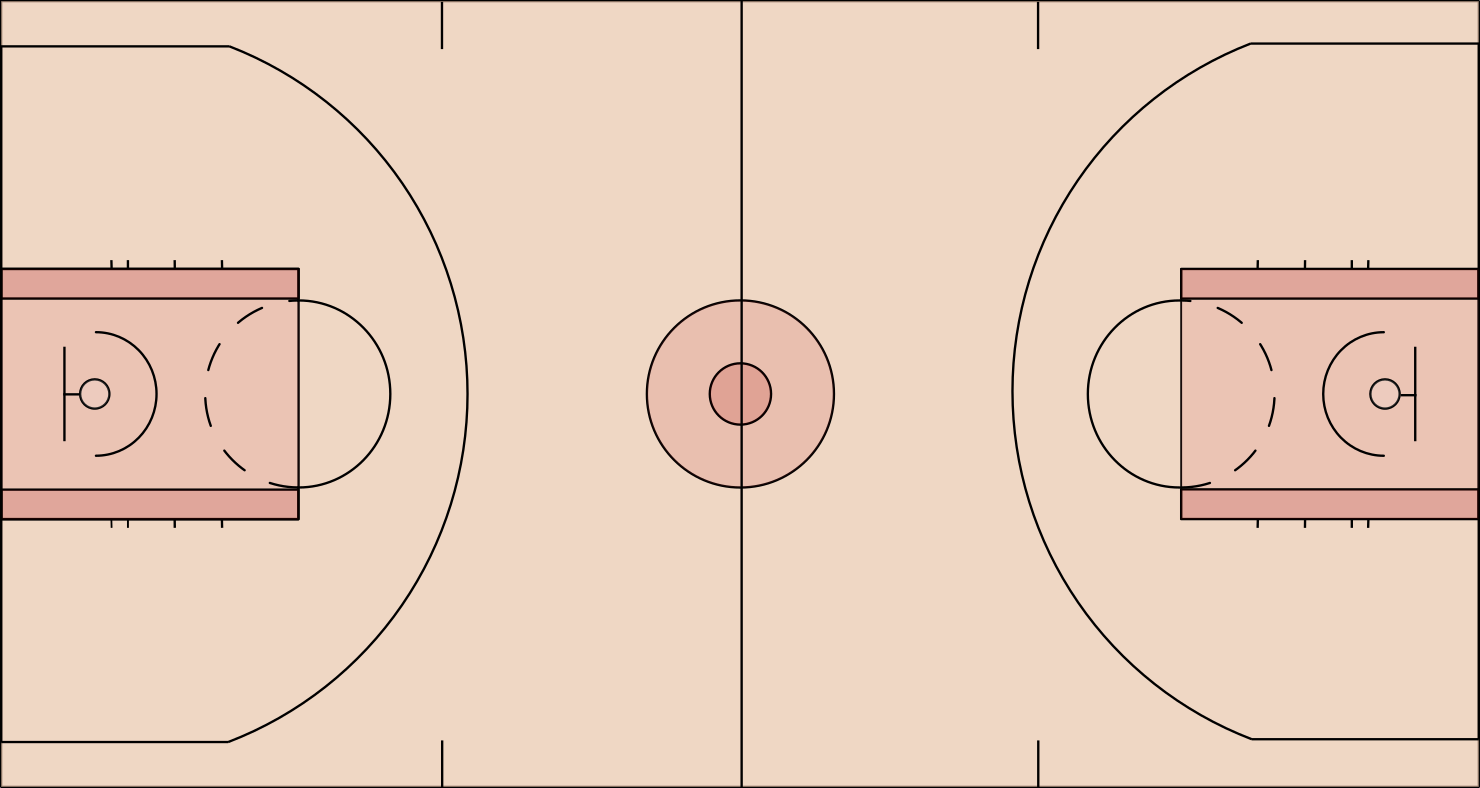
\includegraphics[width=\textwidth]{contents/nba_court.png}
    \caption{Diagram of a typical NBA basketball court.}
    \label{fig:nba_court}
\end{figure}

\paragraph {overview:}
\label{sect:original_nba}

To facilitate the development and validation of these models, this study utilizes a dataset sourced from the ``NBA-Player-Movements'' repository by Linou et al. \cite{linouk}. The dataset contains 636 games from the 2015/16 season. Each game is stored in a compressed ``.7z'' format, which can be extracted using tools such as 7zip. Once extracted, the data is presented in a ``.json'' format, which was further processed using Python to prepare it for analysis. Upon reading the JSON file into a pandas DataFrame, the data is structured with three primary columns: \textbf{``gameid''}, \textbf{``gamedate''}, and \textbf{``events''}. The \textbf{``gameid''} and \textbf{``gamedate''} columns contain the unique identifier for each game and the corresponding date, respectively. These values remain constant for each row (event) within a single game. The \textbf{``events''} column contains detailed information about each individual event, represented as a dictionary. The keys of this dictionary are \textbf{``eventId''}, \textbf{``visitor''}, \textbf{``home''}, and \textbf{``moments''}. Information regarding the \textbf{``visitor''} and \textbf{``home''} keys, which provide details about the teams involved, is discussed in Section \ref{sect:teams}. Details about the \textbf{``moments''} key, which contains information on specific moments within events, will be elaborated on in Section \ref{sect:moments}. Figure \ref{fig:data-structure} provides a graphical representation of the dataset structure, illustrating the organization of the data columns and the relationships between different elements, including the main file structure, team details, and moment details.

\paragraph {Home and Visitor Team:}
\label{sect:teams}

In the dataset, information about both the home and visitor teams is provided under the \textbf{``home''} and \textbf{``visitor''} keys, respectively. Each team is represented as a dictionary that contains several important details. Specifically, the dictionary includes the team's \textbf{``name''}, which is its official designation, the \textbf{``teamid''}, a unique identifier used to distinguish the team from others, and the \textbf{``abbreviation''}, which is a short code representing the team’s name for convenience.

Within each team dictionary, there is a \textbf{``players''} key that points to a list of dictionaries. Each dictionary in this list represents an individual player on the team. For each player, the dictionary includes the \textbf{``lastname''} and \textbf{``firstname''}, which together identify the player. It also includes the \textbf{``playerid''}, a unique identifier for the player, and the \textbf{``jersey''} number, which is unique within the team and indicates the player's number. Lastly, the \textbf{``position''} describes the player’s role on the team, such as forward, center, or guard. Figure \ref{fig:data-structure} shows the structure graphically. 

\paragraph {Moments:}
\label{sect:moments}

The \textbf{``moments''} key in the dataset provides detailed information about specific events within the game. Each entry under this key is a list of \textbf{``moment''}s, where each \textbf{``moment''} contains several pieces of information. These details include the \textbf{``quarter''}, which indicates the quarter number during which the moment occurred, and the \textbf{``moment\_id''}, representing the absolute timestamp of the moment in UNIX format. Additionally, \textbf{``game\_clock''} and \textbf{``shot\_clock''} provide further temporal information, measured in seconds. The \textbf{``None''} field typically remains empty and does not contain any data. The \textbf{``objects''} key within each moment lists the details of all players on the field and the ball, usually totaling 11 entries: 5 players from each team and the ball. For each entry, the data includes \textbf{``teamid''} and \textbf{``playerid''}, which are consistent across all moments. Additionally, \textbf{``x\_pos''} and \textbf{``y\_pos''} provide the positional information of each player in feet, with the origin defined as the lower left corner of the field. The \textbf{``ball\_radius''} is relevant only for the ball, providing its radius, which indirectly gives information about the ball's height or z-axis position. For a visual representation of the structure of these moment details, please refer to Figure \ref{fig:data-structure}.

\begin{figure}[t]
\centering
\includesvg[width=\textwidth]{contents/data-structure.svg}
\caption{Graphical representation of the dataset structure, including the main file (left) and details about the home and vistor teams (center), and moments~(right).}
\label{fig:data-structure}
\end{figure}


\paragraph {Data Preparation and Transformation:}
\label{sect:data-prep}

To create a usable dataset, several preparation steps were undertaken. The complex nested structure described earlier was simplified into a more manageable two-dimensional DataFrame. Each moment was converted into a row, with all relevant information contained within these rows. While this transformation increased disk usage due to the replication of data, such as game dates and game IDs, which were previously represented only once per match, the trade-off was justified by the improved accessibility and ease of use gained through flattening the structure.

Each moment contains data for 11 objects—comprising 5 players from each team and the ball—each with distinct attributes, specifically position and velocity. To streamline the dataset, unnecessary fields were removed, including \textbf{``firstname''}, \textbf{``lastname''}, \textbf{``jersey''}, \textbf{``teamname''}, \textbf{``gamedate''}, and irrelevant fields such as the \textbf{``None''} column. This decision was based on the focus of the task, which required generalizable models rather than identification of individual players or teams. By retaining only the essential data, such as the game name in the filename and removing these extraneous columns, disk space usage was reduced by precisely \(62.30\%\).

The resulting dataset contains, for each moment, the positions (\textbf{x\_pos}, \textbf{y\_pos}) and velocities (\textbf{vx}, \textbf{vy}) of all 10 players and the ball. These positions are specified in feet, with the origin defined at the lower left corner of the court. The velocity data is derived from the positional changes over time and provides crucial information for dynamic~analysis.

The original dataset was recorded primarily in 0.04-second intervals, equating to a sampling rate of 25Hz. However, due to occasional missing data points, some time spans were incomplete. To ensure consistency and maintain the temporal resolution, these gaps were filled using interpolation. Missing values were interpolated to preserve the integrity of the time series data, enabling a seamless analysis of player and ball movements.

To further enhance consistency, the rows were sorted by ascending event numbers and then by \textbf{"moment\_id"} within each event. Additionally, events with fewer than 8 seconds of data (or fewer than 200 \textbf{"moments"}) were excluded to maintain consistency across the dataset and reduce the risk of bias from shorter events, which are typically not useful for many models. After cleaning, the dataset shrank by 36.44\%, resulting in approximately 163,000 remaining events.

The overall reduction in data size, considering both row and column cleaning, was calculated as 
\[
z = 1 - (1 - x)(1 - y) = 1 - (1 - 0.623)(1 - 0.3644) \approx 0.76 
\]
This indicates that more than three-quarters of the original data was ultimately removed during preprocessing. The final dataset is a single two-dimensional DataFrame consisting solely of the unique \textbf{event\_id}, unique \textbf{moment\_id}, and the positions and velocities of all players and the ball.

To prepare the data for model training, the dataset was split into training and validation sets using a 95-5 ratio. All games except the specific game, \textbf{TOR@LAL}, where \textbf{TOR} is the visiting team and \textbf{LAL} is the home team, were included in these sets. This particular game, \textbf{TOR@LAL}, was set aside as the testing dataset. The training and validation sets consist of 6,365 events (2,131,840 moments), with 6,047 events used for training and 318 events for validation. The separate testing dataset comprises 153 events (57,504 moments). This split allows an examination of how well the model generalizes from one team to another, providing insights into its performance and adaptability in various contexts.

\textbf{Velocity Calculation for Each Time Step:}  
To compute the velocity from the positional data provided in the \textbf{``x\_pos''} and \textbf{``y\_pos''} fields at each moment, three differentiation methods are employed, depending on the time step. Special cases are required for the first and last time steps due to the lack of neighboring data points at these boundaries. The calculated velocities are saved as \textbf{``x\_vel''} and \textbf{``y\_vel''} alongside with the index of the player:

\begin{itemize}
    \item \textbf{First Time Step (Forward Differentiation):} For the first time step, velocity is approximated using forward differentiation:
    \[
    v(t_0) = \frac{x(t_1) - x(t_0)}{\Delta t}
    \]
This method is applied because there is no available preceding time step for backward differentiation, necessitating the use of a one-sided differentiation approach.

    \item \textbf{Intermediate Time Steps (Central Differentiation):} For all intermediate time steps, velocity is calculated using central~differentiation:
    \[
    v(t_i) = \frac{x(t_{i+1}) - x(t_{i-1})}{2 \Delta t}
    \]
    This method provides a more accurate approximation of velocity at each intermediate time step \( t_i \) by utilizing both neighboring~points.

    \item \textbf{Last Time Step (Backward Differentiation):} At the final time step, velocity is estimated using backward~differentiation:
    \[
    v(t_n) = \frac{x(t_n) - x(t_{n-1})}{\Delta t}
    \]
    This approach is employed because there is a lack of subsequent data points required for forward differentiation, resulting in the necessity of one-sided differentiation.
\end{itemize}


\subsection{Soccer}
\label{sect:SOC}
Soccer, similar to basketball, is a dynamic and fast-paced sport where two teams compete to control the ball and score goals. Both sports emphasize teamwork, strategy, and quick decision-making, making them useful for testing similar predictive models. However, a key difference lies in the playing field. Unlike the strictly regulated NBA court, which measures approximately 28.65 meters in length and 15.24 meters in width, soccer fields are not uniformly sized across all datasets or competitions. The size of a soccer field can vary significantly, typically ranging between 100-110 meters in length and 64-75 meters in width. This variability in field dimensions can introduce additional complexity when processing soccer data for comparison with basketball data.

To address this, it is crucial to normalize the soccer dataset into the same format as the NBA dataset \ref{sect:NBA} for consistency in analysis and accurate comparison between the two sports. The soccer court dimensions used in this dataset are illustrated in Figure \ref{fig:soccer_court}, which provides a visual representation of the standard field layout and dimensions.

\begin{figure}[t]
    \centering
    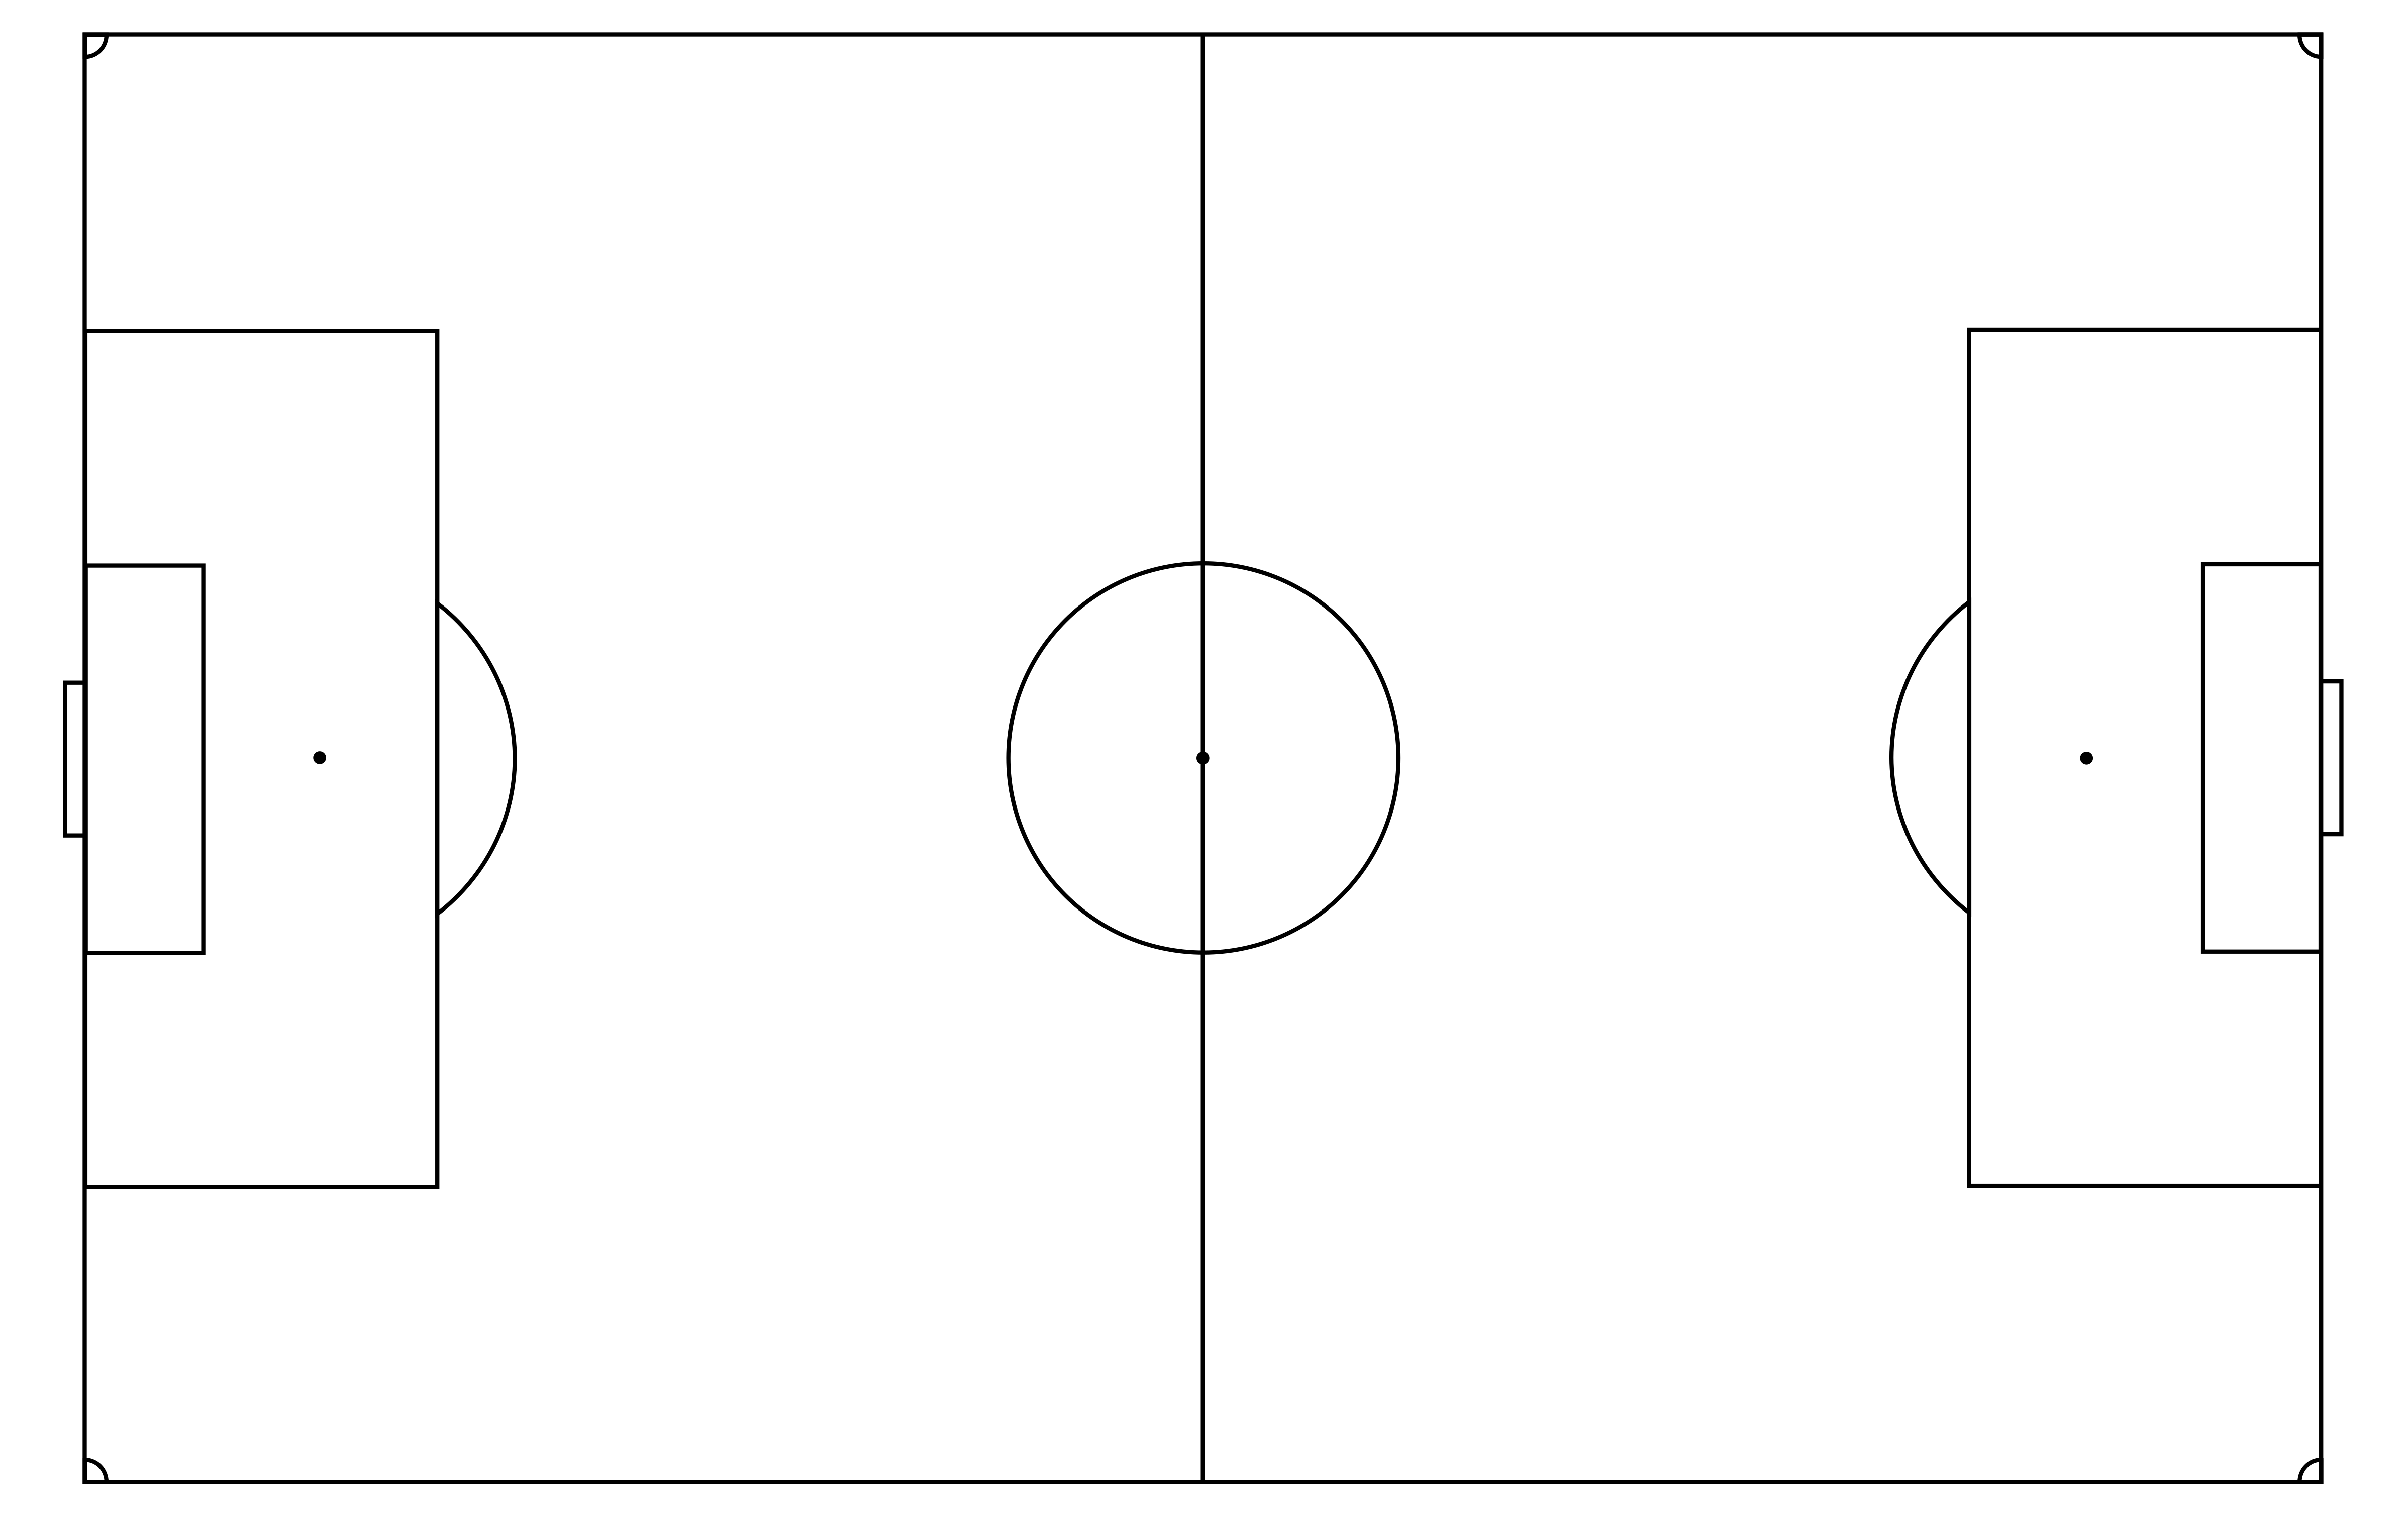
\includegraphics[width=\textwidth]{contents/drawing_rg.png}
    \caption{Diagram of a typical DFL soccer field.}
    \label{fig:soccer_court}
\end{figure}



\paragraph {overview:}
\label{soc:details}
The Soccer dataset consists of 316 games from the Deutsche Fu{\ss}ball Liga (DFL) for the 2014/15 and 2015/16 seasons and was provided by the Fraunhofer Institute for Integrated Circuits IIS. Unlike the original NBA files, the Soccer dataset is flat and straightforward. It is organized into two separate two-dimensional datasets: one for the ball \ref{sect:ball} and one for the players \ref{sect:players}. In this dataset, information about players, teams, and games is replaced with encrypted text to ensure privacy and anonymity.

\paragraph {Ball:}
\label{sect:ball}
The dataset also includes detailed information about the ball at every moment during the game. The relevant fields are \textbf{BallStatus}, \textbf{M}, \textbf{N}, \textbf{Period}, \textbf{S}, \textbf{T}, \textbf{TeamBallPossession}, \textbf{X}, and \textbf{Y}. Specifically, \textbf{BallStatus} indicates the current status of the ball, such as whether it is in play or not. The \textbf{N} column represents the moment identifier, which shows the sequence of recorded moments, and \textbf{M} is the event number within the game. The \textbf{Period} field denotes the current period of the game (e.g., 1st quarter, 2nd quarter), while \textbf{S} provides a timestamp marking the specific moment in seconds since the start of the event. The \textbf{T} field shows the absolute time in milliseconds since the start of the game. The \textbf{TeamBallPossession} indicates which team has possession of the ball at a given moment, and \textbf{X} and \textbf{Y} represent the x and y coordinates of the ball’s position on the court, respectively. Each row in the dataset corresponds to a particular moment, capturing the ball's position and status during that time. In snippet \ref{fig:ball-dataset} , the \textbf{BallStatus} field shows whether the ball is in play. The \textbf{M} column indicates these are sequential moments within the same period of the game. The \textbf{S} field represents the time in seconds within the current event, while \textbf{T} provides the absolute time in milliseconds since the game's start.

The \textbf{TeamBallPossession} field reveals which team had possession of the ball, and the \textbf{X} and \textbf{Y} fields track the ball's movement on the court.

\begin{figure}[H]
    \centering
    \begin{BVerbatim}
    BallStatus,M,N,Period,S,T,TeamBallPossession,X,Y
0,1,10000,1,6.38,1418481028680,DFL-CLU-00000G, 9.85,37.12
1,1,10001,1,6.35,1418481028720,DFL-CLU-00000G, 9.82,37.06
1,1,10002,1,6.36,1418481028760,DFL-CLU-00000G, 9.80,36.99
1,1,10003,1,6.38,1418481028800,DFL-CLU-00000G,10.33,37.37
1,1,10004,1,1.96,1418481028840,DFL-CLU-00000G,10.02,37.29
1,1,10005,1,2.68,1418481028880,DFL-CLU-00000G,10.09,37.44
    \end{BVerbatim}
    \caption{snippet of the Ball dataset for Soccer}
    \label{fig:ball-dataset}
\end{figure}



\paragraph {Players:}
\label{sect:players}

The dataset includes detailed information for each player, captured at every moment within the game. The relevant fields in the dataset are \textbf{M}, \textbf{N}, \textbf{Period}, \textbf{PersonId}, \textbf{PlayingPosition}, \textbf{S}, \textbf{T}, \textbf{TeamId}, \textbf{X}, and \textbf{Y}, which represent crucial attributes of each player. Specifically, \textbf{N} is the moment identifier indicating the sequence of recorded moments, \textbf{M} is the event number within the game, and \textbf{Period} refers to the current period of the game (e.g., 1st quarter, 2nd quarter). The \textbf{PersonId} is a unique identifier for each player, anonymized in this dataset, and \textbf{PlayingPosition} denotes the player's position on the court (e.g., guard, forward). The \textbf{S} field provides a timestamp marking the specific moment in seconds since the start of the event, while \textbf{T} represents the absolute time in milliseconds since the start of the game. The \textbf{TeamId} uniquely identifies the team to which the player belongs, and the \textbf{X} and \textbf{Y} fields capture the x and y coordinates of the player's position on the court. The code snipped \ref{fig:player-dataset} illustrates an example.


\begin{figure}[H]
    \centering
    \begin{BVerbatim}
           M,N,Period,PersonId,PlayingPosition,S,T,TeamId,X,Y
1,10000,1,DFL-OBJ-00001T,IVL,0.00,1418412626360,DFL-CLU-00000F,-26.36, 9.95
1,10001,1,DFL-OBJ-00001T,IVL,2.04,1418412626400,DFL-CLU-00000F,-26.36, 9.96
1,10002,1,DFL-OBJ-00001T,IVL,2.08,1418412626440,DFL-CLU-00000F,-26.36, 9.97
1,10003,1,DFL-OBJ-00001T,IVL,2.05,1418412626480,DFL-CLU-00000F,-26.36, 9.98
1,10004,1,DFL-OBJ-00001T,IVL,1.90,1418412626520,DFL-CLU-00000F,-26.36,10.00
1,10005,1,DFL-OBJ-00001T,IVL,1.90,1418412626560,DFL-CLU-00000F,-26.36,10.01
    \end{BVerbatim}
    \caption{snippet of the Player dataset for Soccer}
    \label{fig:player-dataset}
\end{figure}


\paragraph {Data Preparation and Transformation:}
\label{sect:data-prep-soccer}

For the soccer dataset, a similar preparation process was employed. The data was recorded at 25Hz (0.04-second intervals) and was mostly consistent, with interpolation being used to fill in any missing or erroneous data points. The entire dataset was split into training and validation sets using a 95-5 ratio, while the game \textbf{0002ZV} was used exclusively as the testing dataset. The training and validation sets consist of 2,786 trajectories (4,194,182 moments), with 2,646 trajectories used for training and 140 for validation. The testing dataset contains 88 trajectories (130,711 moments). The dataset was structured to integrate player and ball information into a single, unified format. Each row in the dataset contained all relevant attributes for a specific moment, including positions (\textbf{x\_pos}, \textbf{y\_pos}) and velocities (\textbf{vx}, \textbf{vy}) for both players and the ball. To ensure comprehensive analysis, all these attributes were combined into single rows, allowing for a detailed examination of player and ball dynamics throughout the game. In the process of cleaning the dataset, certain fields were deemed unnecessary for the current study. Specifically, for the ball data, the following keys were removed: \textbf{BallStatus}, \textbf{Period}, \textbf{S}, and \textbf{TeamBallPossession}. For player data, the keys \textbf{Period}, \textbf{PersonID}, \textbf{Playing Position}, \textbf{S}, and \textbf{TeamID} were also excluded. These fields did not contribute to the core analysis and thus were removed to streamline the dataset. To enhance the dataset's utility, velocity information was introduced. Velocity calculations for each time step followed the same differentiation methods as described in the NBA dataset preparation Section (see Section \ref{sect:data-prep}), using forward, central, and backward differentiation techniques depending on the position in the time series.
The final dataset is a two-dimensional DataFrame that integrates the positions and velocities of all players and the ball. All rows contained more than 8 seconds of data, meaning no data was excluded based on duration. However, it was essential to verify this criterion to ensure consistency. This dataset is designed to support detailed analysis and modeling, enabling insights into player behavior, game strategies, and overall dynamics. The structured approach to data preparation ensures that the dataset is both comprehensive and reliable for training and evaluating models.



\section{Experiments}
\label{sec:experiments}

This Section describes the experimental setup designed to address key research questions regarding model performance. Each experiment is tailored to explore a specific aspect of the problem, providing insights that directly answer the research questions posed in this study. The Results of the experiments are shown in Chapter \ref{chapt:results}.

\subsection{E1: Attention-Based versus Baseline Models}
\label{exp:e1}
This experiment addresses Question Q1: \textbf{How do attention-based models compare to other models in general?} We evaluate the performance of attention-based models, particularly the Transformer, against baseline models such as 1LL, 2LL, LSTM, and LMU. All models are trained and tested on the NBA and DFL datasets using the full input context, with \texttt{features\_in} = 4 (velocity and positional information) and the full \SI{2.0}{\second} historical context. The number of objects is \texttt{num\_objects} = 25 for the NBA (2 × 11 players + 1 ball + 2 baskets) and \texttt{num\_objects} = 13 for soccer (2 × 5 players + 1 ball + 2 goals). All models in this Section are multivariate, handling all variables together. The aim is to compare forecasting accuracy, energy consumption, and training time to assess the effectiveness of attention mechanisms in human motion forecasting.

\subsection{E2: Evaluating Impact of Input Exclusions}
\label{exp:e2}
This experiment addresses Question Q2: \textbf{How does model performance vary when positional or velocity data is excluded?} For each model, we assess a version excluding either positional or velocity data, resulting in \texttt{features\_in} = 2 during training and testing. By analyzing the changes in forecasting accuracy and robustness, we aim to determine the impact of each data type on model performance. This investigation will provide insights into the trade-offs between computational efficiency and predictive accuracy, thereby informing optimal input strategies for human motion forecasting.


\subsection{E3: Robustness to Reduced Historical Information}
\label{exp:e3}
This experiment addresses Question Q3: \textbf{How robust is each model to reduced historical information?} We evaluate all models using the full context of \texttt{features\_in} = 4 but with shortened historical lengths. The historical input is reduced from the original \SI{2}{\second} (50 frames) to \SI{1}{\second} (25 frames), \SI{0.4}{\second} (10 frames), and \SI{0.04}{\second} (1 frame) on the \SI{25}{\hertz} dataset. By examining how each model's performance changes with these varying time intervals, we aim to assess their adaptability and accuracy in forecasting human motion with reduced historical data. This analysis will identify which models exhibit greater resilience and reliability when extensive historical context is unavailable.

\subsection{E4: Comparing Univariate and Multivariate Predictors}
\label{exp:e4}
This experiment addresses Question Q4: \textbf{How does a multivariate predictor compare to multiple univariate predictors in terms of forecasting accuracy?} We use the full context with \texttt{features\_in} = 4 and the complete \SI{2}{\second} historical length. In this experiment, we split the x-axis and y-axis into two separate univariate models for each architecture, with one model processing the x-axis data and the other processing the y-axis data. The linear models 1LL and 2LL are not investigated in this case due to a lack of interest. This comparison aims to determine whether the original multivariate models, capable of capturing interactions between axes, outperform their univariate counterparts or if independently processing each axis yields better forecasting accuracy.


\subsection{E5: Generalization Across Different Teams}
\label{exp:e5}
This experiment tackles Question Q5: \textbf{How do the models generalize to other teams?} We evaluate the generalization capabilities of the models using the full input context and historical length. For the NBA dataset, the models are trained solely on the Los Angeles Lakers, with the Toronto Raptors serving as the unseen team for testing. In the soccer dataset, the models are trained only on the anonymized team 00000F, with the anonymized team 0002ZV as the unseen team. This approach allows us to assess how well each model adapts to different team dynamics and behaviors. Understanding the extent to which these models can generalize is crucial for their application in real-world scenarios, where variability in team performance is common.


\subsection{E6: Transfer Learning with Pre-trained Models}
\label{exp:e6}
This experiment addresses Question Q6: \textbf{How does transfer learning impact model performance when trained on one domain and fine-tuned on another?} This analysis is conducted with a reduced input context of one object, specifically including the ball and the basketball/goal information, resulting in \texttt{num\_objects} = 4 per timestep. We will investigate the efficacy of transfer learning by initially training our models on a dataset from one team or sport and then fine-tuning them on a different team or sport. This approach helps evaluate how well the pretrained models adapt to the new context and whether this transfer leads to improved performance. Understanding the benefits of transfer learning is crucial for enhancing model robustness and applicability in diverse team-based sports environments.

\subsection{E7: Evaluating Player Performance in Isolation}
\label{exp:e7}
This experiment addresses Question Q7: \textbf{How does each model perform when predicting the movement of a single target player using only that player's data, excluding the social-interaction context?} In this experiment, we utilize the full input context and length, but the number of players has been reduced to one player per game, resulting in \texttt{num\_objects} = 4 (1 player + 1 ball + 2 baskets for NBA, and 1 player + 1 ball + 2 goals for soccer). We train each model using only the data from the target player, effectively removing the influence of other players' movements. We then evaluate the models' forecasting accuracy based on this limited input. By analyzing the results, we aim to understand the impact of excluding social-interaction information on each model's performance in predicting individual player dynamics.



\section{Model Configurations}
\label{sec:model_configurations}

This Section provides an overview of the configurations used for training each of the six models: 1LL, 2LL, LSTM, LMU, Transformer, and BitNet. Details about the architectures of each model can be found in Section \ref{sec:main_proc}. Here, we list the main hyperparameters used for training, such as hidden size, learning rate, and other relevant configurations for each model. All models were trained using the AdamW optimizer \cite{adamw}, which is known for its effective handling of sparse gradients and improved convergence properties. The learning rate was kept consistent across all models, set to \texttt{learning\_rate} of $0.001$.

\begin{itemize}
    \item \textbf{One Layer Linear Model (1LL):} 
    No additional configurations are provided for the 1LL model (see Section \ref{sec:1ll-details}).
    
    \item \textbf{Two Layer Linear Model (2LL):} 
    The 2LL model (see Section \ref{sec:2ll-details}) has a \texttt{hidden\_size} of $1024$ and a \texttt{dropout\_rate} of $0.1$.
    
    \item \textbf{Long Short-Term Memory Model (LSTM):} 
    The LSTM model (see Section \ref{sec:lstm-details}) has a \texttt{hidden\_size} of $256$ and a \texttt{dropout\_rate} of $0.1$.
    
    \item \textbf{Legendre Memory Unit Model (LMU):} 
    The LMU model (see Section \ref{sec:lmu-details}) has a \texttt{hidden\_size} of $256$, a \texttt{memory\_size} of $256$, and a \texttt{dropout\_rate} of $0.1$. Additionally, the parameters \texttt{learn\_a} and \texttt{learn\_b} are set to true.
    
    \item \textbf{Transformer Model:} 
    The Transformer model (see Section \ref{sec:transformer-details}) employs a convolutional layer as the positional encoder, which has a \texttt{kernel\_size} of $3$, a \texttt{stride} of $1$, and \texttt{padding} of $1$. The Transformer has a \texttt{hidden\_size} of $256$, \texttt{n\_blocks} of $6$, \texttt{n\_heads} of $8$, \texttt{ffn\_hiddens} of $1024$, and a \texttt{dropout\_rate} of $0.1$. Additionally, the Transformer introduces a learning rate warm-up, as described in Section \ref{sec:scheduler}, with 1000 warm-up steps.
    
    \item \textbf{BitNet Model:} 
    Similar to the Transformer model, the BitNet model (see Section \ref{sec:bitnet-details}) employs a convolutional layer as the positional encoder, with a \texttt{kernel\_size} of $3$, a \texttt{stride} of $1$, and \texttt{padding} of $1$. The BitNet has a \texttt{hidden\_size} of $256$, \texttt{n\_blocks} of $6$, \texttt{n\_heads} of $8$, \texttt{ffn\_hiddens} of $1024$, and a \texttt{dropout\_rate} of $0.1$. The BitNet does not include a warm-up scheduler.
\end{itemize}


\section{Training Details}
\label{sec:training_details}

The training details for the main models on the \gls{nba} and \gls{dfl} datasets are presented below. All models were trained with a patience of 20 epochs, and energy consumption was measured using Courty et al.'s CodeCarbon \cite{codecarbon}, an estimation tool for energy usage during training. For both \gls{nba} and \gls{dfl} datasets, the same hyperparameters were utilized, since our aim is to provide a generalizable model, which doesn't have to be configured for each sport separately.

Due to the high memory requirements of attention-based models such as the Transformer and BitNet, a batch size of 16 was used to prevent out-of-memory situations during training. In contrast, other models with lower memory requirements were able to be trained with a larger batch size of 64.

The detailed training metrics for each model are summarized in Table \ref{training_details_nba} for the NBA dataset and Table \ref{training_details_soccer} for the Soccer dataset. These tables provide insights into the following metrics: Parameters in Millions, Model Size in Megabytes (MB), batch size, number of Epochs, Training Loss measured as Mean Squared Error (MSE) in meters, Energy Consumption in milliwatt-hours ($\si{\milli\watt\hour}$), Energy per Epoch (En. per ep.) in milliwatt-hours ($\si{\milli\watt\hour}$), and Training Time (Tr. time) in the format (hh:mm:ss).




\begin{table}[b]
    \centering
    \caption[Table of Training details for NBA Dataset]{This table provides detailed training details of every model for the nba dataset.}
    \begin{tabular}{l||c|c|c|c|c|c}
        \label{training_details_nba}
        \textbf{Metric} & \textbf{1LL} & \textbf{2LL} & \textbf{LSTM} & \textbf{LMU} & \textbf{Trafo} & \textbf{BitNet} \\ \hline \hline
        Params (M) & 0.520 & 2.9 & 0.895 & 0.303 & 4.9 & 4.9 \\ \hline 
        Model Size (MB) & 2.081 & 11.474 & 3.581 & 1.213 & 19.430 & 19.541 \\ \hline 
        batch\_size & 64 & 64 & 64 & 64 & 16 & 16 \\ \hline 
        
        Epochs & 46 & 34 & 82 & 97 & 46 & 79 \\ \hline 
        Train Loss (\si{\meter})& 2.44 & 1.86 & 1.66 & 1.66 & 1.66 & 1.77 \\ \hline
        Energy (\si{\milli\watt\hour}) & 30.05 & 29.04 & 33.53 & 141.85 & 206.02 & 324.54 \\ \hline
        En. per ep. (\si{\milli\watt\hour}) & 0.65 & 0.85 & 0.41 & 1.46 & 4.48 & 4.11 \\ \hline
        Tr. Time (hh:mm:ss) & 00:01:34 & 00:01:28 & 00:08:59 & 02:09:21 & 00:44:15 & 02:46:55 \\ 
    \end{tabular}
\end{table}

\begin{table}[b]
    \centering
    \caption[Table of Training details for Soccer Dataset]{This table provides detailed training details of every model for the Soccer dataset.}    
    \begin{tabular}{l||c|c|c|c|c|c}
    \label{training_details_soccer}
    \textbf{Metric} & \textbf{1LL} & \textbf{2LL} & \textbf{LSTM} & \textbf{LMU} & \textbf{Trafo} & \textbf{BitNet} \\ \hline \hline
    Params (M) & 1.0 & 5.3 & 0.944 & 0.315 & 4.9 & 4.9 \\ \hline 
    Model Size (MB) & 4.001 & 21.304 & 3.777 & 1.263 & 19.578 & 19.688 \\ \hline 
    batch\_size & 64 & 64 & 64 & 64 & 16 & 16 \\ \hline 
    
    Epochs & 70 & 121 & 70 & 129 & 53 & 132 \\ \hline 
    Train Loss (\si{\meter})& 3.37 & 1.82 & 1.08 & 1.01 & 1.08 & 1.27 \\ \hline
    Energy (\si{\milli\watt\hour}) & 19.07 & 20.77 & 27.35 & 131.21 & 107.94 & 192.50 \\ \hline
    En. per ep. (\si{\milli\watt\hour}) & 0.30 & 0.17 & 0.39 & 1.02 & 2.04 & 1.46 \\ \hline
    Tr. Time (hh:mm:ss) & 00:02:03 & 00:04:02 & 00:04:32 & 01:20:06 & 00:25:12 & 02:13:51 \\ 
    \end{tabular}
\end{table}

